\documentclass[Madrid]{beamer}\usepackage[]{graphicx}\usepackage[]{color}
%% maxwidth is the original width if it is less than linewidth
%% otherwise use linewidth (to make sure the graphics do not exceed the margin)
\makeatletter
\def\maxwidth{ %
  \ifdim\Gin@nat@width>\linewidth
    \linewidth
  \else
    \Gin@nat@width
  \fi
}
\makeatother

\definecolor{fgcolor}{rgb}{0.345, 0.345, 0.345}
\newcommand{\hlnum}[1]{\textcolor[rgb]{0.686,0.059,0.569}{#1}}%
\newcommand{\hlstr}[1]{\textcolor[rgb]{0.192,0.494,0.8}{#1}}%
\newcommand{\hlcom}[1]{\textcolor[rgb]{0.678,0.584,0.686}{\textit{#1}}}%
\newcommand{\hlopt}[1]{\textcolor[rgb]{0,0,0}{#1}}%
\newcommand{\hlstd}[1]{\textcolor[rgb]{0.345,0.345,0.345}{#1}}%
\newcommand{\hlkwa}[1]{\textcolor[rgb]{0.161,0.373,0.58}{\textbf{#1}}}%
\newcommand{\hlkwb}[1]{\textcolor[rgb]{0.69,0.353,0.396}{#1}}%
\newcommand{\hlkwc}[1]{\textcolor[rgb]{0.333,0.667,0.333}{#1}}%
\newcommand{\hlkwd}[1]{\textcolor[rgb]{0.737,0.353,0.396}{\textbf{#1}}}%

\usepackage{framed}
\makeatletter
\newenvironment{kframe}{%
 \def\at@end@of@kframe{}%
 \ifinner\ifhmode%
  \def\at@end@of@kframe{\end{minipage}}%
  \begin{minipage}{\columnwidth}%
 \fi\fi%
 \def\FrameCommand##1{\hskip\@totalleftmargin \hskip-\fboxsep
 \colorbox{shadecolor}{##1}\hskip-\fboxsep
     % There is no \\@totalrightmargin, so:
     \hskip-\linewidth \hskip-\@totalleftmargin \hskip\columnwidth}%
 \MakeFramed {\advance\hsize-\width
   \@totalleftmargin\z@ \linewidth\hsize
   \@setminipage}}%
 {\par\unskip\endMakeFramed%
 \at@end@of@kframe}
\makeatother

\definecolor{shadecolor}{rgb}{.97, .97, .97}
\definecolor{messagecolor}{rgb}{0, 0, 0}
\definecolor{warningcolor}{rgb}{1, 0, 1}
\definecolor{errorcolor}{rgb}{1, 0, 0}
\newenvironment{knitrout}{}{} % an empty environment to be redefined in TeX

\usepackage{alltt}
\author{Kayla Janos}
\title{The \emph{googleVis} package}
\date{March 3,2014}
\usepackage{graphicx}
\IfFileExists{upquote.sty}{\usepackage{upquote}}{}
\begin{document}









%Title Slide
\begin{frame}
\maketitle
\end{frame}

%Basic Information Slide
\begin{frame}
\center{\huge{Basic Information}}
\begin{itemize}
\item{To create a \emph{googleVis} chart or graph, you must have a connection to the internet}
\item{This means that unfortunately you can not produce these graphs direction in a \latex document}
\item{Although you have the downfall of not being able to include a \emph{googleVis} product in a \LaTeX document, \emph{googleVis} is a great tool for when your final product is HTML based}
\end{itemize}
\end{frame}
%Chart Types 

\begin{frame}
\center{\huge{Chart Types}}
\begin{itemize}
\item{Annotated Time Line}
\item{Area Chart}
\item{Bar Chart}
\item{Bubble Chart}
\item{Candlestick Chart}
\item{Combo Chart}
\item{Column Chart}
\item{Gauge Chart}
\item{Geo Chart}
\item{Geo Map}
\item{Intensity Map}
\item{Line Chart}
\item{Map}
\item{Motion Chart}
\item{Org Chart}
\item{Pie Chart}
\item{Scatter Chart}
\end{itemize}
\end{frame}

%basic code 
\begin{frame}
\center{\huge{The basic code}}
\begin{itemize}
\item{The commands for each type of chart always begins with \bf{gvis}}
\item{After gvis the next part is the chart type you would like to use}
\item{So for example if you would like to create a pie chart the code would be \emph{gvisPieChart(.....)} with the options you want for your pie chart in the middle}
\begin{itemize}
\item{The chart types will always be capitalized}
\end{itemize}
\end{itemize}
\end{frame}


\begin{frame}
\center{\huge{RStudio and GoogleVis}}
\begin{itemize}
\item{Once your code is written you have to use the plot command on it}
\item{Once it is plotted, you have to the viewer will be blank}
\begin{itemize}
\item{To actually see the vizualization you have to click on the button that opens it in a webpage}
\end{itemize}
\end{itemize}
\end{frame}
\begin{frame}
\center{\Huge{Examples}}
\end{frame}



\begin{frame}
\center{\Huge{Maps}}
\center{\large{Code}}
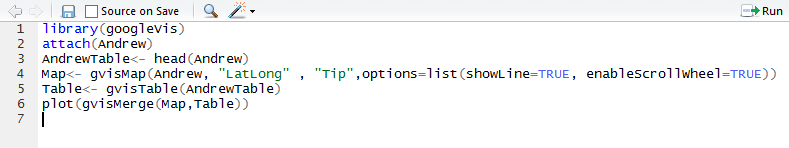
\includegraphics[scale=.5]{MapCode}
\center{\large{Product}} \linebreak
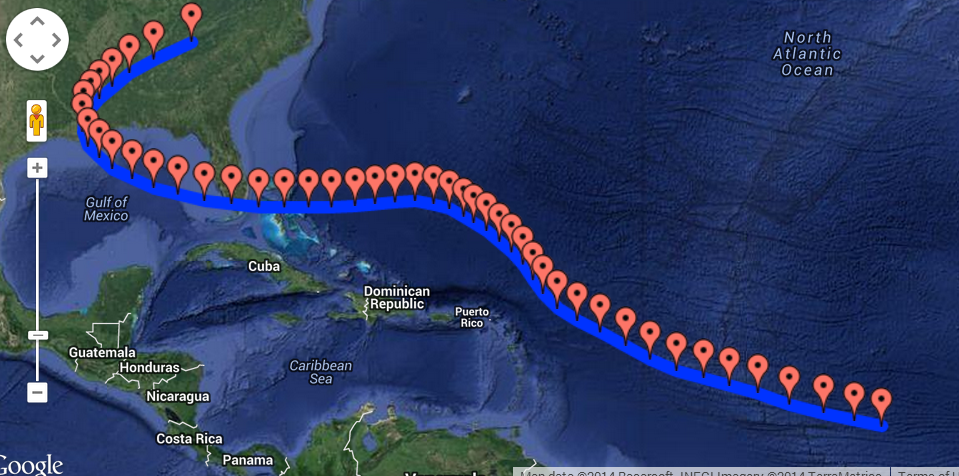
\includegraphics[scale=.35]{map}
\end{frame}

\begin{frame}
\center{\huge{GeoMap}}
\center{\large{Code}}\linebreak
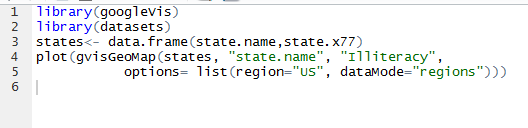
\includegraphics[scale=.45]{geocode} \linebreak
\center{\large{Product}} \linebreak
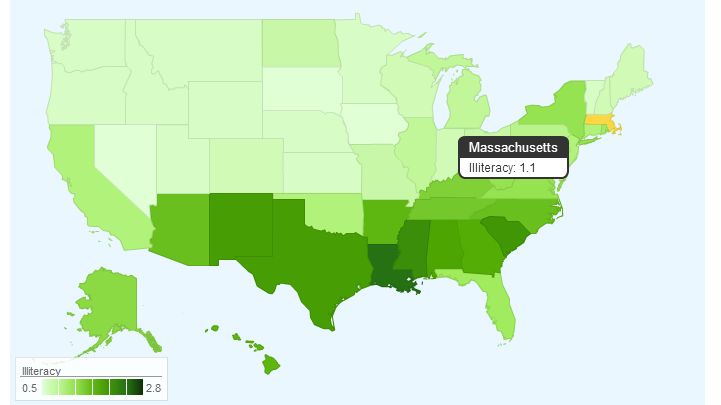
\includegraphics[scale=.5]{geomap}
\end{frame}


\end{document}
